\documentclass[8pt]{beamer}
\usefonttheme[onlymath]{serif}


\setbeamertemplate{frametitle}{%
  \vskip1ex
  \usebeamerfont{frametitle}%
  \insertsubsectionhead\par        %  ← 원하는 대로 변경 가능
  \vskip1ex
  \hrule                             % 밑줄(선택)
}

\setbeamertemplate{blocks}[rounded][shadow=true] % 블록 테두리 둥글게

\setbeamertemplate{itemize item}{\usebeamerfont{itemize item}\textbullet}
\setbeamertemplate{itemize subitem}{\usebeamerfont{itemize subitem}\textbullet}
\setbeamertemplate{itemize subsubitem}{\usebeamerfont{itemize subsubitem}\textbullet}

% 테마 선택 (선택 사항)
% \usetheme{Madrid} % 기본 테마, 다른 테마 사용 가능
% \font{serif}
\usepackage{amsfonts}
\usepackage{amssymb}
\usepackage[T1]{fontenc} % To use combination of textbf, textit
\usepackage[dvipsnames]{xcolor}   % can use more variant colors

% \setcounter{MaxMatrixCols}{20}

% (필요한 패키지들)
% \usepackage{amsthm}
\setbeamertemplate{theorems}[numbered]  % 정리, 정의 등에 번호를 달아줌

% \theoremstyle{plain} % insert bellow all blocks you want in italic
% \newtheorem{theorem}{Theorem}[section] % to number according to section
% 
% \theoremstyle{definition} % insert bellow all blocks you want in normal text
% \newtheorem{definition}{Definition}[section] % to number according to section
% \newtheorem*{idea}{Proof idea} % no numbered block

\newtheorem{proposition}[theorem]{Proposition}

\usepackage{tcolorbox}

% 필요할 경우 패키지 추가
\usepackage{graphicx} % 이미지 삽입을 위한 패키지
\usepackage{amsmath}   % 수식 사용
\usepackage{hyperref}  % 하이퍼링크 추가
\usepackage{cleveref}
\usepackage{multicol}  % 여러 열 나누기
\usepackage{ulem} % 취소선 및줄 나누기
\usepackage{mathtools} % dcases
%\usepackage{xparse} % NewDocumentCommand



% \NewDocumentCommand{\DefThreeOp}{m}{%
%   % \csname #1\endcsname 라는 이름으로, 3개 인자를 받는 새 매크로를 정의
%   \expandafter\NewDocumentCommand\csname #1\endcsname{mmm}{%
%     \operatorname{#1}\!\bigl(##1,\,##2,\,##3\bigr)%
%   }%
% }

\newcommand{\mrm}[1]{\mathrm{#1}}
\newcommand{\mbb}[1]{\mathbb{#1}}
\newcommand{\mb}[1]{\mathbf{#1}}
\newcommand{\mc}[1]{\mathcal{#1}}
\newcommand{\tb}[1]{\textbf{#1}}
\newcommand{\ti}[1]{\textit{#1}}
\newcommand{\Pois}[1]{\operatorname{Pois}(#1)}

\newcommand{\myber}[1]{\operatorname{Bern}\!\left(#1\right)}
\newcommand{\Bin}[2]{\operatorname{Bin}\!\left(#1,#2\right)}
\newcommand{\NBin}[2]{\operatorname{NBin}\!\left(#1,#2\right)}
\newcommand{\mytoinf}[1]{#1 \rightarrow \infty}
\newcommand{\myexp}[1]{\exp{\left(#1\right)}}
\newcommand{\Unif}[2]{\operatorname{Unif}\!\left(#1, #2\right)}
\newcommand{\mygeom}[1]{\operatorname{Geom}\!\left(#1\right)}
\newcommand{\Expo}[1]{\operatorname{Expo}\!\left(#1\right)}
\newcommand{\abs}[1]{\left\lvert #1 \right\rvert}
\newcommand{\floor}[1]{\left\lfloor #1 \right \rfloor}
\newcommand{\expec}[1]{\operatorname{E}\left[ #1 \right]}
\newcommand{\Var}[1]{\operatorname{Var}\left[#1\right]}
\newcommand{\myskew}[1]{\operatorname{Skew}\!\left[#1\right]}
\newcommand{\mykurt}[1]{\operatorname{Kurt}\!\left[#1\right]}
\newcommand{\mywei}[2]{\operatorname{Wei}\!\left(#1, #2\right)}
\newcommand{\Span}{\operatorname{Span}}
\newcommand{\Cov}[2]{\operatorname{Cov}\!\left(#1, #2\right)}
\newcommand{\intinfty}{\int_{-\infty}^\infty}
\newcommand{\Corr}[2]{\operatorname{Corr}\!\left(#1, #2\right)}
\newcommand{\Mult}[3]{\operatorname{Mult}_{#1}\!\left(#2, #3\right)}
\newcommand{\Beta}[2]{\operatorname{Beta}\!\left(#1, #2\right)}
\newcommand{\HGeom}[3]{\operatorname{HGeom}\!\left(#1, #2, #3\right)}
\newcommand{\NHGeom}[3]{\operatorname{NHGeom}\!\left(#1,#2, #3\right)}
\newcommand{\GammaDist}[2]{\operatorname{Gamma}\!\left(#1, #2\right)}
%\DefThreeOp{PHGeom}

\newcommand{\im}{\operatorname{im}}
\newcommand{\tr}{\operatorname{tr}}


% 발표 제목, 저자, 날짜 설정
\title{Introduction to Mathematical Analysis: The Structure of the Real Numbers: Sequences}
\author{Gwanwoo Choi}
% \date{}

\begin{document}
% 표지 슬라이드

\begin{frame}
    \titlepage
\end{frame}

\subsection{Completeness of the Real Numbers}
\begingroup
    \setbeamertemplate{frametitle}{%
    \vskip1ex
    \usebeamerfont{frametitle}%
    \insertframetitle\par        %  ← 원하는 대로 변경 가능
    \vskip1ex
    \hrule                             % 밑줄(선택)
    }
    \begin{frame}
        \frametitle{Table of Contents}
        \tableofcontents[currentsubsection]
    \end{frame}
\endgroup

% % 목차 슬라이드

\begin{frame}{.}
    \begin{definition}
        A nonempty set $S$ of real numbers is said to be \tb{bounded above} if there exists some real number $M$ such that $x \leq M$ for every $x$ in $S$.
        In this case $M$ is said to be an \tb{upper bound} for $S$.
        Likewise, $S$ is said to be \tb{bounded below} if there exists some number $m$ such that $m \leq x$ for all $x$ in $S$.
        $m$ is called a \tb{lower bound} for $S$.
        We call $S$ \tb{bounded} if it is both above and below.
    \end{definition}

    \begin{definition}
        Let $S$ be a nonempty set of real numbers that is bounded above.
        A \tb{supremum} or \tb{least upper bound} of $S$, denoted $\sup S$, is a real number $\mu$ such that
        \begin{enumerate}
            \item $x \leq \mu$, for all $x \in S$
            \item If $M$ is an upper bound for $S$, then $\mu \leq M$
        \end{enumerate}

        An \tb{infimum} or \tb{greatest lower bound} of $S$, denoted $\inf S$, is a real number $\nu$ such that
        \begin{enumerate}
            \item $\nu \leq x$, for all $x \in S$
            \item If $m$ is any lower bound for $S$, then $\nu \geq m$
        \end{enumerate}
    \end{definition}
\end{frame}

\begin{frame}{.}
    \begin{example}
        Consider the open interval $S = (a,b) = \{x \mid x \in \mbb{R}, a < x < b\}$.
        Note that for any $a<x<b$, $(x+b)/2 \in S$, so $x$ is not an upper bound of $S$.
        Also, for any $a<x<b$, $(x+a)/2 \in S$, so $x$ is not a lower bound of $S$.
        So $\inf S = a$ and $\sup S = b$.
    \end{example}


    \begin{block}{Archimedes' Principle}
        Let $\epsilon$ and $M$ be any two positive real numbers.
        There exists a $k$ in $\mbb{N}$ such that $M < k \epsilon$.
    \end{block}

    \begin{example}
        Let $S = \{(-1)^k \left(1 - \frac{1}{k}\right) | \forall k \in \mbb{N} \} = \{0, 1/2, -2/3, 3/4, -4/5, \dots\}$.
        Then $S$ is bounded and upper bound is $1$ and lower bound is $-1$.
        Note that $10, 100$ also can be upper bound and $-10, -100$ can be lower bound.

        Let assume there exists another upper bound $x$ such that $x < 1$.
        Then by Archimedes' principle, there exists a $k \in \mbb{N}$ such that $1 < (2k)(1-x)$.
        Then $x$ satisfies $x < 1 - \frac{1}{2k} = (-1)^{2k} (1 - \frac{1}{2k})$.
        Note that $(-1)^{2k} (1 - \frac{1}{2k}) \in S$.
        So $x$ is not an upper bound of $S$ and $1$ becomes to leaset upper bound of $S$.
    \end{example}
\end{frame}

\begin{frame}{.}
    \begin{block}{Bernoulli's Inequality (Exercise 1.16)}
        \begin{itemize}
            \item  For all $x > -1$ and all $n \in \mbb{N}$, $(1+x)^n \geq 1 + nx$ holds. (\underline{Bernoulli's inequality})

            \ti{Proof.} $n=1$ case is trivial.
            Let assume the equation holds when $n=k$.
            Then $(1+x)^k \geq 1+ kx$ holds.
            Then $(1+x)^{k+1} \geq (1+kx)(1+x) = 1 + (k+1)x + kx^2 \geq 1 + (k+1)x$

            \item For any $\mu > 0, \mu \in \mbb{R}$ and $k \in \mbb{N}$, $1 < \mu k \implies (\mu - \frac{1}{k})^n \geq \mu^n - \frac{n \mu^{n-1}}{k}$ holds.
            $1 < \mu k \implies 1 > \frac{1}{\mu k}$. So, by Bernoulli's inequality, $(1 - \frac{1}{\mu k})^n \geq  1 + n(-\frac{1}{\mu k}) \implies (\mu - \frac{1}{k})^n \geq \mu^n - \frac{n \mu^{n-1}}{k}$ holds.
        \end{itemize}
    \end{block}

    \begin{example} \label{ex:1}
        Fix $r >1$ and let $S = \{r^k \mid k \in \mc{N}\}$.
        The claim is $S$ is not bounded above and hence $\sup S$ does not exist in $\mbb{R}$.
        Let $r = 1+c$ for some $c >0$.
        Then by Bernoulli's inequality, $r^k = (1+c)^k \geq 1+kc$ holds.

        Let assume $M \in \mbb{R}, M >0$ and $M$ is upper bound of $S$.
        Then by Archimedes' principle, ther exists a $k$ such that $M - 1 < kc$.
        Then $M < 1+kc \leq (1+c)^k = r^k$ and $M$ is not an upper bound of $S$.
    \end{example}

    Example \ref{ex:1} shows that there can exist a nonempty set that is not bounded above.
\end{frame}

\begin{frame}{.}
    The all-important question arises: If $S$ is bounded above, does $\sup S$ exist?

    \begin{example}
        Let $S$ be the closed interval $S = [a,b] = \{x \mid x \in \mbb{R}, -\sqrt{2} \leq x \leq \sqrt{2}\}$.
        Then it is trivial that $\sup S = \sqrt{2}$ and $\inf S = -\sqrt{2}$.
        Note that $\sup S, \inf S \in \mbb{R}$.

        Now let $S^\prime = [a,b] = \{x \mid x \in \mbb{Q}, -\sqrt{2} \leq x \leq \sqrt{2}\}$.
        but in this time $\sup S, \inf S \notin \mbb{Q}$.

        This implies $\mbb{R}$ is more complete than $\mbb{Q}$.
    \end{example}


    \begin{block}{Axiom: The Completeness Axiom for $\mbb{R}$}
        If $S$ a non-empty set of real numbers that is bounded above, then $\exists \sup S \in \mbb{R}$.
    \end{block}

\end{frame}

\begin{frame}{.}
    \begin{example}
        Fix $c>0$ and $n \in \mbb{N}$.
        Let $S = \{x \mid x \in \mbb{R}, 0 <x^n <c \}$.

        First show that $S$ is non-empty.
        Since $c >0$, by Archimedes' principle, there exists a $k \in \mbb{N}$ such that $1 < ck$.
        Then $1 < ck \leq ck^n \implies 1 < ck^n \implies 1/k^n < c$.
        This implies $1/k \in S$ and $S \neq \emptyset$.

        Is $S$ bounded above?
        Choose any $M > \max (c,1)$.
        Then $0 < x^n < c < M < M^n \implies x < M$.
        So $S$ is upper bound of $S$.

        By axiom, $\exists \sup S \in \mbb{R}$.
        Let $\mu = \sup S$.
        Intuitively we now that $\mu^n = c$.
        So we want to show that $\mu^n < c$ or $\mu^n >c$ are impossible.

        First, let assume $\mu^n < c$.
        Let $M = \sum_{j=1}^n \binom{n}{j} \mu^{n-j}$.
        Since $(c - \mu^n) >0, M >0$, by Archimedes' principle, there exists a $k \in \mbb{N}$ such that $M < k (c - \mu^n) \implies M/k < (c - \mu^n)$.
        Let expand $(\mu + 1/k)^n = \sum_{j=0}^n \binom{n}{j} \mu^{n-j} (1/k)^j = \mu^n + (1/k)\sum_{j=1}^n \binom{n}{j} \mu^{n-j} (1/k)^{j-1} \leq \mu^n + 1/k \sum_{j=1}^n \binom{n}{j} \mu^{n-j} = \mu^n + M/k \leq \mu^n + (c - \mu^n) =c$.
        This shows that $(\mu + 1/k) \in S$ (contradiction!).
        
        Suppose that $\mu^n > c$. Then $\exists k \in \mbb{N}$  such that $1 < \mu k, n \mu^{n-1} < (\mu^n -c) k$. By Bernoulli's inequality, $(mu - \frac{1}{k})^n \geq \mu^n - \frac{n \mu^{n-1}}{k} > \mu^n - (\mu^n - c) = c > x^n$.
        So $\mu - \frac{1}{k}$ must be an upper bound for $S$ (contradiction!).

        $\therefore \mu = c^{\frac{1}{n}}$.
    \end{example}
\end{frame}

\begin{frame}{.}
    \begin{block}{Exercise 1.19}
        Prove by induction that, for every $j \in \mbb{N}$, $2^{j-1} \leq j!$.

        If $j=1$, $2^0 = 1 \leq 1! = 1$.
        Suppose for $k \in \mbb{N}$, $2^{k-1} \leq k!$ holds.
        Then $2^k \leq 2 \cdot k! \leq (k+1)\cdot k! \leq (k+1)!$.
    \end{block}


    \begin{example}
        Let $S = \{x_k = \sum_{j=0}^k \frac{1}{j!} \mid \forall k \in \mbb{N}\}$.
        The claim is that $S$ is bounded above.
        For any $k$, $x_k = 1 + \frac{1}{1!} + \frac{1}{2!} + \cdots + \frac{1}{k!} \leq 1 + \frac{1}{2^0} + \frac{1}{2^1} + \cdots + \frac{1}{2^{k-1}} = 1 + \frac{1 - \frac{1}{2}^k}{1 - \frac{1}{2}} = 1 + 2\left(1 - \frac{1}{2}^k\right) <3$.
        So, $S$ is bounded above by $3$.
        By axiom, $\exists \sup S \in \mbb{R}$ and $\sup S = e$.
    \end{example}
\end{frame}

\begin{frame}{.}
    We can observe following facts from Several examples
    \begin{itemize}
        \item $\mu = \sup S$ may or may not belong to $S$.
        \item Whenever $\mu$ is in $S$, $\mu$ is the maximum of $S$.
        \item If $S$ has a largest element $M$, then $M = \sup S$.
    \end{itemize}

    \begin{theorem} \label{th:1}
        Let $S$ be a non-empty set  of real numbers and let $\mu$ and $\nu$ be real numbers.
        \begin{enumerate}
            \item Suppose that $S$ is bounded above. Then $\mu = \sup S$ if and only if $\mu$ is an upper bound for $S$ and, for every $\epsilon >0$, there exists an $x \in S$ such that $\mu - \epsilon < x \leq \mu$.
            \item Suppose that $S$ is bounded below. Then $\nu = \inf S$ if and only if $\nu$ is a lower bound for $S$ and, for every $\epsilon > 0$, there exists an $x \in S$ such that $\nu \leq x < \nu + \epsilon$.
        \end{enumerate}

        Proof.

        (1. $\implies$) Suppose there were no point of $S$ in the interval $(\mu - \epsilon,\mu]$ for any $\epsilon >0$.
        Then $\mu-\epsilon$ would be an upper bound for $S$ and this is contradiction.
        So there exists a point of $S$ in the interval $(\mu - \epsilon, \mu]$.

        (1. $\impliedby$) Suppose there exists an upper bound $M < \mu$.
        Let $d = \mu - M$.
        Then for $d >0$, there should exist a point $x \in S$ such that $\mu - d = M < x \leq \mu$.
        Then $M$ is not an upper bound of $S$ and this is contradiction.
    \end{theorem}
\end{frame}

\begin{frame}{.}
    \begin{block}{Exercise 1.5}
        Use the Axiom and theorem \ref{th:1} to derive Archimedes' principle.

        For any $\epsilon > 0$, let $S = \{k\epsilon \mid \forall k \in \mbb{N}\}$.
        Suppose that $S$ is bounded above.
        Then by axiom, $\exists \mu = \sup S$.
        By theorem \ref{th:1}, there exists a point $k\epsilon$ in the interval $\mu - \epsilon < k \epsilon \leq \mu$.
        In left-hand side, $\mu < (k+1)\epsilon$ and $(k+1) \epsilon \in S$.
        So $\mu$ is not an upper bound for $S$ (contradiction!).

        So the assumption, $S$ is bounded above, is false.

        This means for any large positive constant $M$, $\exists k\epsilon$ such that $M < k \epsilon$.
    \end{block}

    \begin{block}{Exercise 1.6}
        Show that Archimedes' principle is equivalent to the following statement: For any $c > 0$, there exists a $k \in \mbb{N}$ such that $k-1 \leq c <k$.

        ($\implies$) Let $\epsilon = 1$ and $M = c > 0$.
        Then $c < k$ holds for some $k \in \mbb{N}$.
        Note that there exists many $k$s.
        Let $k_0$ be the smallest one such that $c < k_0$.
        Then $c < k_0$ holds but $c <k_0 -1$ not holds.
        Then we can rewrite as $k_0 -1 \leq c <k_0$.

        ($\impliedby$) Let $c = \frac{M}{\epsilon}$.
        Then there exists a $k$ such that $k-1 \leq \frac{M}{\epsilon} < k$.
        Then in the right-side, $M < \epsilon k$ holds.
    \end{block}
\end{frame}

\begin{frame}{.}
    \begin{theorem} \label{th:3}
        Between any two real numbers there is a rational number.

        Proof.

        Suppose $c, d \in \mbb{R}$ such that $0 < c< d$.
        Since $d -c >0$, by Archimedes' principle, $\exists q \in \mbb{N}$ satisfies $1 < (d-c) q$.
        That is, $cq +1 < dq$.
        Since $cq > 0$, $\exists p \in \mbb{N}$ such that $p- 1\leq cq < p$.
        Combining, $p-1 \leq cq < p  \leq cq + 1 < dq$.
        $\therefore cq < p <dq \implies c < p/q < d$.

        (Exercise 1.7) Let prove for $c < d \leq 0$ case.
        By Archimedes' principle, $\exists q \in \mbb{N}$ that satisfies $1 < (d-c) q$.
        Then $1 + cq < dq$ holds.
        Also, $\exists p \in \mbb{N}$ such that $p-1 \leq - cq < p$.
        Then $-p < cq \leq 1-p$.
        Combining, $-p < cq \leq 1 -p < 1+cq < dq \implies cq < 1-p <dq \implies c < \frac{1-p}{q} < d$.

        Let prove for $c \leq 0 < d$ case.
        By Archimedes' principle, $\exists q \in \mbb{N}$ $1 < dq$.
        Then $c \leq 0 < \frac{1}{q} < d$.
    \end{theorem}
\end{frame}

\begin{frame}{.}
    \begin{block}{Exercise 1.10} \label{exercise:1.10}
        Suppose that $c$ is a real number such that, for all $\epsilon >0$, it is true that $\abs{c} < \epsilon$.
        Prove that $c$ must be $0$.
    \end{block}

    \begin{block}{Exercise 1.17}
        Prove that if $x$ and $y$ are positive numbers such that $x^n < y^n$ for some $n \in \mbb{N}$, then $x < y$.
        (We say that the taking of positive $n$th roots \ti{preserves order} on $\mbb{R}^+$.)
    \end{block}

    \begin{block}{Exercise 1.20}
    \end{block}
\end{frame}

\subsection{Neighborhoods and Limit Points}

\begingroup
    \setbeamertemplate{frametitle}{%
    \vskip1ex
    \usebeamerfont{frametitle}%
    \insertframetitle\par        %  ← 원하는 대로 변경 가능
    \vskip1ex
    \hrule                             % 밑줄(선택)
    }
    \begin{frame}
        \frametitle{Table of Contents}
        \tableofcontents[currentsubsection]
    \end{frame}
\endgroup

\begin{frame}{.}
    \begin{definition}
        Let $x$ be any real number.
        A \tb{neighborhood} of $x$ with positive radius $r$ is the set $N(x;r) = \{y \in \mbb{R} \mid \abs{y-x} < r \}$.

        A \tb{deleted neighborhood} of $x$ in $\mbb{R}$, denoted $N^\prime (x;r)$, is the neighborhood $N(x;r)$ with the point $x$ itself removed.
    \end{definition}
    When the magnitude of the radius $r$ is immaterial, we will omit mention of it and merely write $N(x)$ and $N^\prime(x)$ to denote a neighborhood and deleted neighborhood of $x$, respectively, of the point $x$.

    \begin{definition}
        Given a nonempty set $S \in \mbb{R}$, a point $x \in \mbb{R}$ is said to be a \tb{limit point} of $S$ if, for each $\epsilon > 0$, the deleted neighborhood $N^\prime(x; \epsilon)$ contains at least one point of $S$.
    \end{definition}
    A limit point $x$ of $S$ is also called an \ti{accumulation point} of $S$ because points of $S$ accumulate near $x$ or a \ti{cluster point} of $S$ because points of $S$ cluster around $x$.
\end{frame}

\begin{frame}{.}
    \begin{example}
        Let $S = \{(-1)^k \cdot (1+\frac{1}{k}) \mid \forall k \in \mbb{N}\} = \{-2, \frac{3}{2}, \frac{-4}{3}, \dots\}$.
        Then $1$ and $-1$ are each limit points of $S$.

        Let's see that 1 is a limit point of $S$.
        By Archimedes' principle, for any $\epsilon>0$, we can choose $k \in \mbb{N}$ such that $\frac{1}{2k} < \epsilon$.
        Then $1<1 + \frac{1}{2k} < 1 + \epsilon$.
        Therefore, $1 + \frac{1}{2k} = (-1)^{2k} (1 + \frac{1}{2k}) \in N^\prime(1; \epsilon) \cap S$ so $N^\prime(1;\epsilon) \cap S$.
        So, $1$ is limit point of $S$

        By similar way, one can show that $-1$ is limit point of $S$.
        Note that neither $1$ nor $-1$ is not point of $S$.
    \end{example}

    \begin{theorem} \label{th:2}
        Let $S$ be a non-empty set in $\mbb{R}$.
        Then a point $x$ is a limit point of $S$ if and only if there is an $\epsilon_0 > 0$ such that, for all $\epsilon$ with $0 < \epsilon < \epsilon_0$, the set $N^\prime(x;\epsilon)$ contains at least one point of $S$.

        ($\implies$) Choose any $\epsilon_0 > 0$ such that, for all $\epsilon$ with $0 < \epsilon < \epsilon_0$, the set $N^\prime (x; \epsilon)$ contains at least one point of $S$.

        ($\impliedby$) Let $\epsilon_1$ be any positive number.
        We have to show that $N^\prime(x; \epsilon_1) \neq \emptyset$.
        For $\epsilon = \min(\epsilon_0, \epsilon_1)$, by the hypothesis $N^\prime(x; \epsilon) \cap S \neq \emptyset$ and $N^\prime(x; \epsilon) \subset N^\prime(x; \epsilon_1)$ holds.
        Therefore $N^\prime(x; \epsilon_1) \neq \emptyset$ and $x$ is a limit point of $S$.
    \end{theorem}
\end{frame}

\begin{frame}{.}
    \begin{example} \label{ex:2}
        Let $a$ and $b$ be real numbers with $a < b$ and let $S=(a,b)$.
        Every point in $[a,b]$ is a limit point of $S$.
        It is trivial that if $x$ is any point in $(a,b)$ and $\epsilon$ is any positive number, then $N^\prime(x;\epsilon)$ contains point of $S$ and $x$ is limit point.

        Let's show that $b$ is limit point of $S$.
        Fix any $\epsilon_0 > 0$ such that $\epsilon_0 < b-a$.
        Then for any $\epsilon >0$ such that $0 < \epsilon < \epsilon_0$, $N^\prime(b; \epsilon) \cap S = (b-\epsilon, b) \neq \emptyset$.
        So by theorem \ref{th:2}, $b$ is a limit point of $S$.

        Similarly, $a$ is a limit point of $S$.
    \end{example}

    \begin{example}
        As a variant of \ref{ex:2}, let $a$ and $b$ be real numbers with $a<b$.

        Fix any $x$ in $(a,b)$ and any positive $\epsilon_0 < \min(x-a, b-x)$.
        Choose any $0 < \epsilon < \epsilon_0$.
        By \ref{th:3}, there is a rational number in the interval $(x-\epsilon, x)$ (and, by the way, also another in $(x, x+\epsilon)$).
        Hence, $N^\prime(x;\epsilon)$ contains a point of $S$.

        By theorem \ref{th:2}, $x$ is a limit point of $S$.

        The endpoints are treated similarly.
    \end{example}
\end{frame}

\begin{frame}{.}
    \begin{example}
        Let $\mbb{Z}$ has no limit points in $\mbb{R}$.

        To prove this, if $k$ is any integer, $0 < \epsilon_0 <1$, and $\epsilon < \epsilon_0$, then $N^\prime(k; \epsilon)$ is contained entirely in $(k-1, k) \cup (k, k+1)$, a set of devoid of integers.
        Thus $k$ cannot be a limit point of $\mbb{Z}$.

        If $x$ is not an integer, then $x \in (\floor{x}, \floor{x}+1)$.
        Note that there is no integer in $(\floor{x}, \floor{x}+1)$.
        If we choose a positive $\epsilon_0 < 
        min(x - \floor{x}, \floor{x}+1 - x)$ and $\epsilon < \epsilon_0$, then $N^\prime(x;\epsilon)$ has no integer.
        Thus $x$ cannot be a limit point of $\mbb{Z}$ either.

        That is, no point of $\mbb{R}$ is a limit point of $\mbb{Z}$.
    \end{example}

    \begin{definition}
        If a non-empty set $S$ in $\mbb{R}$ has no limit points, then $S$ is said to be \tb{discrete}.
    \end{definition}
\end{frame}

\begin{frame}{.}
    \begin{theorem}[The Bolzano-Weierstrass Theorem] \label{th:4}
        If $S$ is a bounded, infinite subset of $\mbb{R}$, then $S$ has a limit point in $\mbb{R}$.

        \smallskip
        \text{}
        Proof.
        Since $S$ is bounded, by Axiom $\nu = \inf S, \mu = \sup S$ exist.
        Clearly, $S \subseteq [\nu, \mu]$.
        Let $c_0 = (a_0 + b_0)/2$.
        Then either $[a_0, c_0]$ or $[c_0, b_0]$ contains infinitely many points of $S$, for otherwise $S$ would be a finite set.
        Let $I_1 =[a_1, b_1]$ denote whichever of the intervals $[a_0, c_0]$ or $[c_0, b_0]$ contains infinitely many points of $S$.
        Note that $I_1 \subset I_0$ and that the length of $I_1$ is $(b_0 - a_0)/2$.

        Let $c_1 = (a_1 + b_1)/2$ and again select $I_2 = [a_2, b_2]$ by similar way.
        Continue this procecure, repeatedly bisecting each interval $[a_k, b_k]$ and choosing $I_{k+1} = [a_{k+1}, b_{k+1}]$ to be the half of $[a_k, b_k]$ that contains infinitely many points of $S$.

        In this way, we can obtain $T = \{I_k \mid \forall k \in \mbb{N}\}$ of closed intervals with the following properties:
        For each $k \in \mbb{N}$, (1.) $S \cap I_k$ is infinite (2.) $I_{k+1} \subset I_k$ (3.) The length of $I_k$ is $b_k - a_k = (b_0 - a_0)/ 2^k$.

        From this fact, for any $k \in \mbb{N}$ and $m \geq k, m \in \mbb{N}$, $a_0 \leq a_k \leq a_m \leq b_m \leq b_k \leq b_0$ holds (the reason why this equation is exercise!).
        Let $A = \{a_k \mid \forall k \in \mbb{N}\}$ be the set of all left endpoints of the intervals $I_k$ and $B = \{b_k \mid \forall k \in \mbb{N}\}$.

        Since neither $A$ nor $B$ is empty and $A$ is bounded above by $b_0$ and $B$ is bounded below by $a_0$, by Completeness Axiom for $\mbb{R}$, $\exists \alpha = \sup A \in \mbb{R}, \exists \beta = \inf B \in \mbb{R}$.

        \underline{The claim is $\alpha = \beta$ and this common value is a limit point of $S$}.
    \end{theorem}
\end{frame}

\begin{frame}{.}
    \begin{block}{Con't}
        Let first see that $\alpha \leq \beta$ and after see that $\alpha = \beta$.
        For every $k=0, 1, \dots,$, $a_k$ is a lower bound for $B$ since $a_k \leq a_m \leq b_m$.
        Therefore, $a_k \leq \beta = \inf B$, $\forall k$.
        Since for all $k$, $a_k \leq \beta$, $\beta$ is also upper bound of $A$. Thus, $\alpha \leq \beta$.

        Let's see that $\alpha = \beta$.
        Now we know that $\forall k, a_k \leq \alpha \leq \beta \leq b_k$.
        Thus $\beta - \alpha \leq b_k - a_k = (b_0 - a_0)/2^{k}$, for all $k$.

        For arbitrary $\epsilon > 0$, we can use Archimedes' principle and an inductive proof to choose a $k \in \mbb{N}$
        such that $ \frac{b_0- a_0}{2^k} \leq \frac{b_0 - a_0}{k} <\epsilon$.
        So, $0 < \beta - \alpha \leq \frac{b_0-a_0}{2^k} < \epsilon$ holds.
        By exercise 1.10, $\beta - \alpha$ should be $0$ and $\alpha = \beta$.

        Let $x_0 = \alpha = \beta$.
        Now we see that $x_0$ is limit point.
        Assign any positive value to $\epsilon$.
        By Archimedes' principle, choose a $k$ in $\mbb{N}$ such that $ b_k - a_k = (b_0 - a_0)/2^k <\epsilon$.
        Then combining with $a_k \leq x_0 \leq b_k$, $x_0 + \epsilon > x_0 + (b_k - a_k) = b_k - (x_0 - a_k) \leq b_k$ holds.
        Also, $x_0 - \epsilon < x_0 - (b_k - a_k) = a_k - (b_k - x_0) \leq a_k$ holds.
        So, $a_k, b_k \in N^\prime(x_0; \epsilon)$. and there exists infinitely many points of $S$ between $a_k$ and $b_k$.

        $\therefore x_0$ is the limit point of $S$ and there always exists a limit point of bounded non-empty set $S$.
    \end{block}

    \begin{definition}
        We say that a nonempty set $X$ has the \tb{Bolzano-Weierstrass property} if every bounded infinite subset $S$ of $X$ has a limit point in $X$. 
    \end{definition}
\end{frame}

\begin{frame}{.}
    \begin{block}{Exercise 1.23}
        Suppose that $S$ is a bounded, infinite subset of $\mbb{R}$.
        Let $\mu = \sup S$.
        Is $\mu$ necessarily a limit point of $S$?
        If so, show that, for every $k \in \mbb{N}$ there exists a point $x \in S$ such that $\mu - \frac{1}{k} < x \leq \mu$.
        If not, exhibit a bounded, infinite set $S \in \mbb{R}$ whose supremum is not a limit point of $S$.

        Let $S = \{1/2^k \mid \forall k \in \mbb{N}\}$.
        Then $\mu = 1/2$.
        Let $\epsilon = \frac{1}{8}$.
        Then there is no element of $S$ in $N^\prime(1/2; 1/8)$.

        Therefore there is no guarantee that $\mu$ is a limit point.
    \end{block}

    \begin{block}{Exercise 1.25}
        If $x$ is any nonzero number and if $0 < \epsilon < \abs{x}$, prove that only finitely many numbers of the form $(-1)^k/2^k$ are in $N(x;\epsilon)$.

        If $x>0$, then for any $\epsilon > 0$, there exists $k \in \mbb{N}$ such that $1 < k (x - \epsilon) < 4^k (x - \epsilon)$.
        This implies $1\ 2^{2m} < x - \epsilon$ for $m \geq k, m \in \mbb{N}$.
        Else if $x < 0$, for any $\epsilon$ s.t. $ 0 < \epsilon < \abs{x}$, $-(x+\epsilon) >0$ and by Archimedes' principle, there exists $k$ such that $1 < -(x+\epsilon) k  < -(x+\epsilon) 2^{2k+1}$.
        Then $x + \epsilon < -1/2^{2k+1}$.
        Then $\forall m \in \mbb{N}, m > k$, $x + \epsilon < -1/2^{2m+1} <0$ holds.

        $\therefore N(x; \epsilon)$ only contains finite points.
    \end{block}
\end{frame}

\begin{frame}{.}
    \begin{block}{Exercise 1.26}
        Prove that a nonempty finite set has no limit points.

        Let order the element of any nonempty finite set $S$, and denote $i$-th element as $x_i$
        Then for $k \in \mbb{N}$, $x_k < x_{k+1}$ holds.

        First, let's see that each $x_i$ is not a limit point.

        Let $d_i = \min(\abs{x_i - x_{i-1}}, \abs{x_i - x_{i+1}})$ if both $x_{i-1}$ and $x_{i+1}$ exist else assign distance with nearest element to $d_i$.
        If we choose $\epsilon> 0$ such that $\epsilon<d_i$, then there is no element in $N^\prime(x_I; \epsilon)$.

        Let me prove that $x$ such that $x_i < x < x_{i+1}$ is not a limit point.
        $d_i = \min(x-x_{i}, x_{i+1} - x)$ and for $0 < \epsilon <d_i$, there is no element in $N^\prime(x; \epsilon)$.

        So there is no limit point for nonempty finite set.s
    \end{block}

    \begin{block}{Exercise 1.29}
        Suppose that $S$ is an unbounded, infinite set in $\mbb{R}$.
        Does $S$ necessarily have a limit point?
        If so, prove it.
        If not, prove an example of an unbounded, infinite set having no limit points.

        $\mbb{Z}$ is good example of an unbounded, infinite set who has no limit points.
    \end{block}
\end{frame}

\begin{frame}{.}
    \begin{block}{Example 1.30}
        Suppose that $S$ is a bounded, infinite subset of $\mbb{R}$ having exactly one limit point $x_0$.
        Prove that, for any $\epsilon >0$, the neighborhood $N^\prime(x_0; \epsilon)$ contains all but finitely many of the points of $S$.

        Suppose to the contrary that $(N^\prime(x_0; \epsilon))^\mathsf{c}$ contains infinitely many points of $S$.
        That is, $S \cap (N^\prime(x_0; \epsilon))^\mathsf{c}$ is an infinite set.
        Since $S$ is a bounded set, its subset $s \cap (N^\prime(x_0 ; \epsilon))^\mathsf{c}$ is also a bounded set.
        So by theorem \ref{th:4}, $S \cap (N^\prime(x_0; \epsilon))^\mathsf{c}$ must have a limit point.
        This is contradiction.
        $\qed$
    \end{block}
\end{frame}

\subsection{The Limit of a Sequence}

\begingroup
    \setbeamertemplate{frametitle}{%
    \vskip1ex
    \usebeamerfont{frametitle}%
    \insertframetitle\par        %  ← 원하는 대로 변경 가능
    \vskip1ex
    \hrule                             % 밑줄(선택)
    }
    \begin{frame}
        \frametitle{Table of Contents}
        \tableofcontents[currentsubsection]
    \end{frame}
\endgroup

\begin{frame}{.}
    The english world \tb{eventually} means "beyond some point in time".
    If you think of the indices $1,2,3,\dots$ as a premitive model for time, then \ti{eventually} translates into the following mathematical phrase: \underline{There exists an index $k_0 \in \mbb{N}$ such that, if $k \geq k_0$...}
    Some state $P(k)$ that depends on $k$ is \ti{eventually} valid if there exists a $k_0$ such that, for $k \geq k_0$, $P(k)$ holds true.

    \smallskip
    Similarly, the english world \tb{frequently} will be translated into the phrase: \underline{For every index $k\in\mbb{N}$, there is at least one $k_1 > k$ such that...}
    We will say that $P(k)$ is \ti{frequently} valid if, for every $k \in \mbb{N}$, there exists at least one $k_1 > k$ such that $P(k_1)$ holds true.

    \smallskip
    Clearly, if a statement $P(k)$ is eventually valid, then it is frequently valid.

    \begin{definition}
        We say that $c$ is a \tb{cluster point} of the sequence $\{x_k\}$ if, for every $\epsilon> 0$ and every $k \in \mbb{N}$, there is a $k_1 > k$ such that $x_{k_1} \in N(c; \epsilon)$.
    \end{definition}

    Put briefly, $c$ is a cluster point of $\{x_k\}$ if terms of the sequence are frequently arbitrary near $c$.
    Note that a limit point of the set $S = \{x_1, x_2, \dots\}$ is automatically a cluster point of the sequence $\{x_k\}$.

    \underline{Note that in definition of cluster point, neighborhood is used instead of deleted} 
    \underline{neighborhood}.
\end{frame}

\begin{frame}{.}
    \begin{example} \label{ex:3}
        Let $x_k = (-1)^k, \forall k \in \mbb{N}$.
        Then the set $S$ is simply $\{-1, 1\}$, consisting of two points and having no limit points.
        But both $-1$ and $1$ are cluster points of the sequence $\{x_k\}$.
    \end{example}

    \begin{definition}
        The sequence $\{x_k\}$ \tb{converges} to $x_0$ and we say that $x_0$ is the \tb{limit} of $
        \{x_k\}$ if, for each neighborhood $N(x_0; \epsilon)$, there exists an index $k_0$ such that, whenever $k \geq k_0$, $x_k$ is in $N(x_0; \epsilon)$.
        We write $\lim_{k \to \infty} x_k = x_0$.
        If a sequence $\{x_k\}$ fails to converge, for whatever reason, then we say that it \tb{diverges}.
    \end{definition}

    Note that
    \begin{itemize}
        \item In definition of convergence of sequence, \ti{neighborhood} is used and contrastly, in definition of limit of set, \ti{deleted neighborhood} is used.
        \item Also, convergence of sequences requires all $x_k$, where $k \geq k_0$, should satisfies $x_k \in N(x_0; \epsilon)$. Instead, in limit point of set, for any $\epsilon > 0$, it accept only one point of $S$ in $N(x_0; \epsilon)$.
    \end{itemize}

\end{frame}

\begin{frame}{.}
    \begin{theorem}
        The limit of a convergent sequence in $\mbb{R}$ is unique.

        proof. we have to prove that $\{x_k\}$ converges to both $x_0$ and $x_0^\prime \implies x_0 = x_0^\prime$.
        Let assume $x_0 = x_0^\prime$.
        Then by choosing $0 < \epsilon < \abs{x_0 - x_0^\prime}/2$, we will obtain a contradiction.
        Since $\lim_{k \to \infty} x_k = x_0$, we can choose $k_1 \in \mbb{N}$ such that $\forall k \geq k_1, x_k \in N(x_0; \epsilon)$.
        Similarly, we can choose $k_2 \in \mbb{N}$ such that, $\forall k \geq k_2, x_k \in N(x_0^\prime; \epsilon)$.

        Let $k_0 = \max(k_1, k_2)$.
        Then $k_0 \in N(x_0; \epsilon)$ and $k_0 \in N(x_0^\prime; \epsilon)$.
        So, $\abs{x_0 - x_0^\prime} = \abs{x_0 - x_k + x_k - x_0^\prime} \leq \abs{x_0 - x_k} + \abs{x_k - x_0^\prime} < \epsilon + \epsilon = 2\epsilon$.
        But by assumption, $2\epsilon < \abs{x_0 - x_0^\prime}$ and this is contradiction because $\abs{x_0 - x_0^\prime} < \abs{x_0 0 x_0^\prime}$ could not be hold.
        $\qed$
    \end{theorem}

    \begin{theorem} \label{th:6}
        If a sequence has two (or more) cluster points, then it must diverge.

        \smallskip
        Our next result provides a logical fulcrum on which many of our subsequent arguments will hinge.
    \end{theorem}

    Recall that \ref{ex:3} has \underline{two cluster points} and therefore \underline{diverges}.
    

\end{frame}

\begin{frame}{.}
    \begin{figure}
        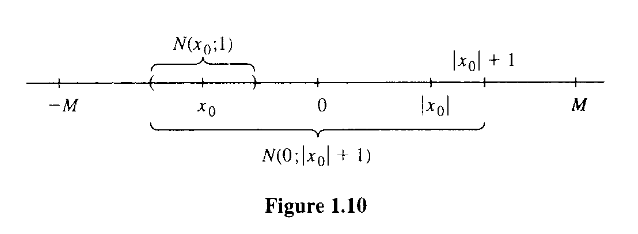
\includegraphics[width=0.7\textwidth]{theorem1.3.3.png}
    \end{figure}

    \begin{theorem} \label{th:5}
        A convergent sequence is bounded.

        \smallskip
        Proof. Suppose that $\{x_k\}$ converges to $x_0$.
        We must show that there exists some real number $M$ such that $\abs{x_k} \leq M$, for $k=1,2,3,\dots$.
        Let $\epsilon=1$.
        Since $\{x_k\}$ converges to $x_0$, $\exists k_0 \in \mbb{N}$ such that $\forall k \geq k_0, k_0 \in N(x_0; 1)$.
        Then $\abs{x_k} = \abs{x_k - x_0 + x_0} \leq \abs{x_k - x_0} + \abs{x_0} < 1 + \abs{x_0}$.
        This implies $x_k \in N(0; 1+\abs{x_0})$.

        Consider the $k_0$ numbers: $\abs{x_1}, \abs{x_2}, \dots, \abs{x_{k_0 - 1}}$ and $\abs{x_0} + 1$.
        We let $M$ be any real number greater than the maximum of these $k_0$ numbers.
        It is easy to see that $\{x_k\}$ must be contained in $N(0;M)$ and is therefore bounded.
        $\qed$
    \end{theorem}
\end{frame}

\begin{frame}{.}
    The contrapositive of \ref{th:5} provides us with the following useful fact.
    \begin{theorem}
        If a sequence is unbounded, then it must diverge
    \end{theorem}

    \begin{example}
        For each $k \in \mbb{N}$, let $x_k = \frac{1}{k}$.
        Intuitively, it is evident that $\lim_{k \to \infty} x_k = 0$.

        By fixing any $\epsilon > 0$ and choosing the smallest positive integer $k_0$ such that $1 < k_0 \epsilon$, $0 < \frac{1}{k_0} < \epsilon$ holds.
        For any $k \geq k_0$ such that $\abs{x_k - 0} = \frac{1}{k} \leq \frac{1}{k_0} < \epsilon$ holds.
        So, $x_k \in N(0; \epsilon)$.

        Thus, $\lim_{k \to \infty} x_k = 0$.
    \end{example}

    \begin{example}
        For each $k \in \mbb{N}$, let $x_k = 1 - \frac{1}{2^k}$.
        We claim that $\lim_{k \to \infty} x_k = 1$.

        Fix $\epsilon > 0$.
        Then $\exists k_0 \in \mbb{N}$ such that $1 < k_0\epsilon < k \epsilon$ where $k \geq k_0$.
        This implies $1 < k\epsilon < 2^k \epsilon \implies \frac{1}{2^k} < \epsilon$.
        Then $\abs{x_k - 1} = \abs{1 - \frac{1}{2^k} -1} = \frac{1}{2^k} < \epsilon$ holds.
        In other words, $x_k \in N(1;\epsilon)$.

        This proves $\lim_{k \to \infty} (1 - \frac{1}{2^k}) = 1$.
    \end{example}
\end{frame}

\begin{frame}{.}
    \begin{figure}
        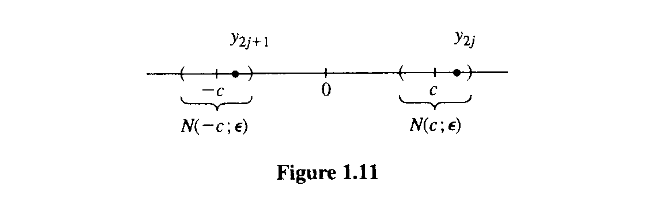
\includegraphics[width=0.75\textwidth]{example1.3.15.png}
    \end{figure}
    \begin{example}
        Let $\{x_k\}$ be any sequence that converges to $0$ and let $c$ be any positive number.
        Let $y_k = (-1)^k(c+x_k)$.
        We claim that both $c$ and $-c$ are cluster points of $\{x_k\}$ and that the sequence must diverge.

        \underline{Claim: both $-c$ and $c$ are cluster points of $\{y_k\}$ and these sequence must divergence}.

        Let fix $0< \epsilon < c$. Then $\exists k_0$ such that $\forall k \geq k_0, \abs{x_k} < \epsilon$.
        Then even $k$, i.e. $k=2j$, $\abs{y_k - c} = \abs{c + x_k - c} = x_k < \epsilon$.
        Also, odd $k$, i.e. $k=2j+1$, $\abs{y_k - (-c)} = \abs{-c -x_k + c} = x_k < \epsilon$.

        Since $\{y_k\}$ has two cluster points, $\{y_k\}$ must diverge by theorem \ref{th:6}.
    \end{example}
\end{frame}

\begin{frame}{.}
    \begin{example}
        For each $k \in \mbb{N}$, define $x_k = \frac{k}{k+1}$.
        Evidently, $\lim_{k \to \infty} x_k = 1$.

        Fix $\epsilon > 0$. We want to show that, eventually, $\abs{x_k -1} = \abs{\frac{k}{k+1} - 1} < \epsilon$ or, equivalently, that $1 - \epsilon < \frac{k}{k+1} < 1 + \epsilon$.
        Since $\frac{k}{k+1} < 1+\epsilon$ is trivial, we only need to show that $1 - \epsilon < \frac{k}{k-1} \implies 1 - \epsilon < k\epsilon$.
        So, we set $k_0 \in \mbb{N}$ as smallest number which satisfies $\frac{1-\epsilon}{\epsilon} < k_0$.
        We want to confirm that, for any $k \geq k_0, x_k \in N(1;\epsilon)$.
        Then $k\epsilon > 1 - \epsilon \implies k - k(1 - \epsilon) > 1-\epsilon \implies k > (k+1)(1-\epsilon) \implies \frac{k}{k+1} > 1- \epsilon$.

        $\therefore x_k \in N(1;\epsilon)$ and $\lim_{k \to \infty} x_k = 1$.
    \end{example}

    \begin{theorem}
        A sequence $\{x_k\}$ converges to $0$ iff $\{\abs{x_k}\}$ converges to $0$ also

        ($\implies$): trivial

        ($\impliedby$): Fix $\epsilon >0$ and $k_0 \in N$ such that for $k \geq k_0$, $\abs{x_k} \in N(0; \epsilon)$.
        This implies $-\epsilon < x_k < \epsilon$ and $x_k \in N(0; \epsilon)$.
    \end{theorem}
\end{frame}

\begin{frame}{.}
    \begin{example}
        Fix any $r$ such that $-1 < r < 1$.
        Clam that $\lim_{k \to \infty} r^k = 0$.
        We only proof for $0< r< 1$.
        We need to exhibit an index $k_0$ with the property that, if $k \geq k_0$, then $r^k \in N(0; \epsilon)$.

        Let $c = \frac{1}{r} -1$.
        Then $r = \frac{1}{1+c}$.
        Note that $r^k = \frac{1}{(1+c)^k} \leq \frac{1}{1 + ck} < \frac{1}{ck}$.

        Fix $\epsilon >0$.
        Then there exists smallest $k_0 \in \mbb{N}$ such that $\frac{1}{c k_0} < \epsilon$.
        For $k \geq k_0$, $r^k < \frac{1}{ck} \leq \frac{1}{c k_0} < \epsilon$.
        This implies $r^k \in N(0;\epsilon)$.
    \end{example}

    \begin{theorem}
        If $\{x_k\}$ converges to $x_\infty$ and if $c$ is any constant, then $\{cx_k\}$ converges to $cx_\infty$.
    \end{theorem}

    \begin{theorem}
        A bounded, monotone sequence of real numbers converges
    \end{theorem}

    Above theorem is an alternative form of Completeness Axiom for $\mbb{R}$
\end{frame}

\begin{frame}{theorem}


\end{frame}


\end{document}